\documentclass[14pt, a4paper]{extarticle}
\title{Functions \& Interval Notation}
\usepackage[a4paper, papersize={8.5in, 120in}, total={7.5in, 120in}]{geometry}
\usepackage{setspace}
\usepackage{amsmath}
\usepackage{amssymb}
\usepackage{changepage}
\usepackage{tikz}
\usepackage{pgfplots}

\author{Jacob Zante}
\date{September 9th, 2024}
\doublespacing
\pgfplotsset{width=7in, compat=newest}
% \usepgfplotslibrary{external}

\begin{document}
\maketitle
\setlength{\parindent}{0pt}



\textbf{1. State the domain and range}
\begin{adjustwidth}{1cm}{0pt}
    \begin{math}
        \textbf{a)} \\
        \text{D: } \{x \in \mathbb{R}\} \\
        \text{R: } \{y \in \mathbb{R} | -4 \leq y \leq -2\} \\
        \\
        \textbf{b)} \\
        \text{D: } \{x \in \mathbb{R} | -1 \leq x \leq 7\} \\
        \text{R: } \{y \in \mathbb{R} | -3 \leq y \leq -1\} \\
        \\
        \textbf{c)} \\
        \text{D: } \{1, 2, 3, 4\} \\
        \text{R: } \{-5, 4, 7, 9, 11\} \\
        \\
        \textbf{d)} \\
        \text{D: } \{x \in \mathbb{R}\} \\
        \text{R: } \{y \in \mathbb{R}\} \\
        \\
        \textbf{e)} \\
        \text{D: } \{-4, -3, 1, 2\} \\
        \text{R: } \{0, 1, 2, 3\} \\
        \\
        \textbf{f)} \\
        \text{D: } \{x \in \mathbb{R}\} \\
        \text{R: } \{y \in \mathbb{R} | y \leq 0\} \\
        \\
    \end{math}
\end{adjustwidth}

\textbf{2. State the domain and range, then deterine whether the relation is a function, and justify your answer.}
\begin{adjustwidth}{1cm}{0pt}
    \begin{math}
        \textbf{a)} \hspace{3.5mm} y = -2(x + 1)^2 - 3 \\
        \text{D: } \{x \in \mathbb{R}\} \\
        \text{R: } \{y \in \mathbb{R} | y \leq -3\} \\
        \text{This relation is a function, as it passes the vertical line test.} \\
        \\
        \textbf{b)} \hspace{3.5mm} y = \frac{1}{x + 3} \\
        \text{D: } \{x \in \mathbb{R} | x \neq -3\} \\
        \text{R: } \{y \in \mathbb{R} | y \neq 0\} \\
        \text{This relation is a function, as it passes the vertical line test.} \\
        \\
        \textbf{c)} \hspace{3.5mm} y = 2^{-x} \\
        \text{D: } \{x \in \mathbb{R}\} \\
        \text{R: } \{y \in \mathbb{R} | y > 0\} \\
        \text{This relation is a function, as it passes the vertical line test.} \\
        \\
        \textbf{d)} \hspace{3.5mm} y = \cos x + 1 \\
        \text{D: } \{x \in \mathbb{R}\} \\
        \text{R: } \{y \in \mathbb{R} | -1 \leq y \leq 1\} \\
        \text{This relation is a function, as it passes the vertical line test.} \\
        \\
        \textbf{e)} \hspace{3.5mm} x^2 + y^2 = 9 \\
        \text{D: } \{x \in \mathbb{R} | -3 \leq x \leq 3\} \\
        \text{R: } \{y \in \mathbb{R} | -3 \leq y \leq 3\} \\
        \text{This relation is not a function, as it does not pass the vertical line test.} \\
        \\
        \textbf{f)} \hspace{3.5mm} y = 2\sin x \\
        \text{D: } \{x \in \mathbb{R}\} \\
        \text{R: } \{y \in \mathbb{R} | -2 \leq y \leq 2\} \\
        \text{This relation is a function, as it passes the vertical line test.} \\
        \\
    \end{math}
\end{adjustwidth}

\textbf{3. Determine whether each relation is a function, and state its domain and range.}
\begin{adjustwidth}{1cm}{0pt}
    \begin{math}
        \textbf{a)} \\
        \text{This relation is a function, because each x value only cooresponds to one y value.} \\
        \text{D: } \{1, 3, 5, 7\} \\
        \text{R: } \{2, 4, 6\} \\
        \\
        \textbf{b)} \\
        \text{This relation is a function, because each x value only cooresponds to one y value.} \\
        \text{D: } \{0, 1, 2, 5\} \\
        \text{R: } \{-1, 3, 6\} \\
        \\
        \textbf{c)} \\
        \text{This relation is a function, because each x value only cooresponds to one y value.} \\
        \text{D: } \{0, 1, 2, 3\} \\
        \text{R: } \{2, 4\} \\
        \\
        \textbf{d)} \\
        \text{This relation is not a function, because there is a value of x that cooresponds to more than one y value.} \\
        \text{D: } \{2, 6, 8\} \\
        \text{R: } \{1, 3, 5, 7\} \\
        \\
        \textbf{e)} \\
        \text{This relation is not a function, because there is a value of x that cooresponds to more than one y value.} \\
        \text{D: } \{1, 10, 100\} \\
        \text{R: } \{0, 1, 2, 3\} \\
        \\
        \textbf{f)} \\
        \text{This relation is a function, because each x value only cooresponds to one y value.} \\
        \text{D: } \{1, 2, 3, 4\} \\
        \text{R: } \{1, 2, 3, 4\} \\
        \\
    \end{math}
\end{adjustwidth}

\textbf{4. Determine whether each relation is a function, and state its domain and range.}
\begin{adjustwidth}{1cm}{0pt}
    \begin{math}
        \textbf{a)} \\
        \text{This relation is a function, as it passes the vertical line test.} \\
        \text{D: } \{x \in \mathbb{R}\} \\
        \text{R: } \{y \in \mathbb{R} | y \geq 2\} \\
        \\
        \textbf{b)} \\
        \text{This relation is not a function, as it does not pass the vertical line test.} \\
        \text{D: } \{x \in \mathbb{R} | x \geq 2\} \\
        \text{R: } \{y \in \mathbb{R}\} \\
        \\
        \textbf{c)} \quad x^2 = 2y + 1 \\
        \text{This relation is a function, as when you isloate for y,} \hspace{2mm} y = 2(x^2 - 1) \hspace{2mm} \text{it becomes clear that there is only one possible y value for every x value.} \\
        \text{D: } \{x \in \mathbb{R}\} \\
        \text{R: } \{y \in \mathbb{R} | y \geq -2\} \\
        \\
        \textbf{d)} \quad x = y^2 \\
        \text{This relation is not a function, as when you isolate for y,} \hspace{2mm} y = \pm \sqrt{x} \hspace{2mm} \text{it becomes clear that there are two possible y values for every x value (positive and negative).} \\
        \text{D: } \{x \in \mathbb{R} | x \geq 0\} \\
        \text{R: } \{y \in \mathbb{R}\} \\
        \\
        \textbf{e)} \quad y = \frac{3}{x} \\
        \text{This relation is a function, as there is only one possible y value for every x value.} \\
        \text{D: } \{x \in \mathbb{R} | x \neq 0\} \\
        \text{R: } \{y \in \mathbb{R} | y \neq 0\} \\
        \\
        \textbf{f)} \quad f(x) = 3x + 1 \\
        \text{This relation is a function, as there is only one possible y value for every x value.} \\
        \text{D: } \{x \in \mathbb{R}\} \\
        \text{R: } \{y \in \mathbb{R}\} \\
        \\
    \end{math}
\end{adjustwidth}

\textbf{7. The following table give's Tina's height above the ground while riding a Ferris wheel, in relation to the time she was riding it.} \\ \\
\begin{tabular}{| c | c | c | c | c | c | c | c | c | c | c | c | c | c |}
    \hline
    Time(s) & 0 & 20 & 40 & 60 & 80 & 100 & 120 & 140 & 160 & 180 & 200 & 220 & 240 \\
    \hline
    Height(m) & 5 & 10 & 5 & 0 & 5 & 10 & 5 & 0 & 5 & 10 & 5 & 0 & 5 \\
    \hline
\end{tabular}
\\

% example: https://www.overleaf.com/project/66e33de5239d635d030d4610
\begin{adjustwidth}{1cm}{0pt}
    \textbf{a) Draw a graph of the relation, using time as the independent variable and height as the dependent variable.} \\
    \begin{adjustwidth}{-1cm}{0pt}
        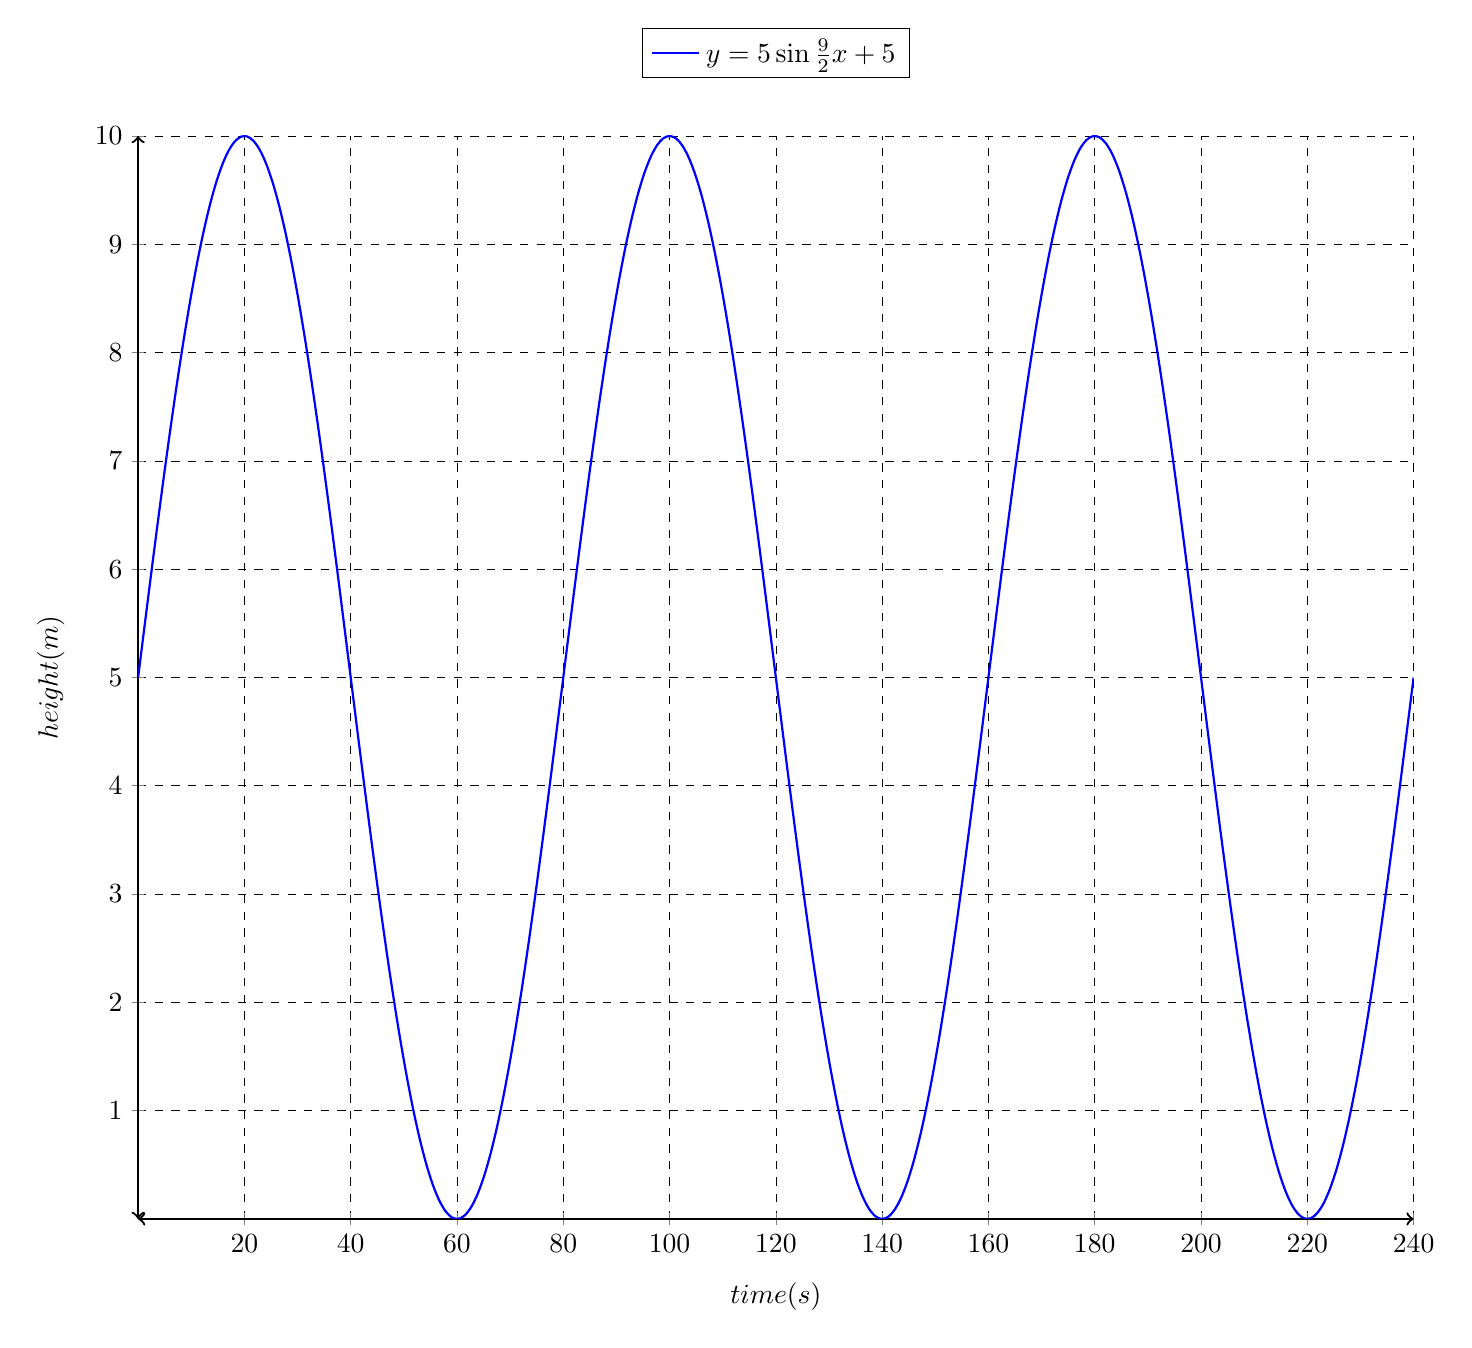
\begin{tikzpicture}
            \begin{axis}[
                axis lines=middle,
                axis line style={thick,<->},
                xmin=0,xmax=240,ymin=0,ymax=10,
                ytick={+1,+2,...,+10},
                xtick={+20,+40,...,+240},
                tick label style={font=\normalsize},
                grid=major,
                major grid style={dashed,very thin,black},
                every axis plot post/.append style={thick},
                label style={font=\normalsize},
                x label style={at={(axis description cs:0.5,-0.05)},anchor=north},
                y label style={at={(axis description cs:-0.05,0.5)},rotate=90,anchor=south},
                xlabel=$time(s)$,
                ylabel=$height(m)$,
                smooth,
                legend style={
                        font=\normalsize,
                        at={(0.5, 1.1)},
                        anchor=north
                        }
                ]
                \addplot[domain=0:240,samples=200,blue]{5 * sin(4.5*x) + 5};
                \legend{$y=5\sin\frac{9}{2}x + 5$}
            \end{axis}
        \end{tikzpicture}
    \end{adjustwidth}
    
    \textbf{b, c) What is the domain? What is the range?} \\
    \begin{math}
        \text{D: } \{x \in \mathbb{R} | 0 \leq x \leq 240\} \\
        \text{R: } \{y \in \mathbb{R} | 0 \leq y \leq 10\} \\
    \end{math}
    \\
    \textbf{d) Is this relation a function? Justify your answer.}\\
    \text{This relation is a function, as it passes the vertical line test.} \\
    \\
    \textbf{e) Another student sketched a graph, but used height as the independent variable. What does this graph look like?} \\
    \begin{math}
        x=5\sin\frac{9}{2}y + 5 \\
        x - 5 = 5\sin\frac{9}{2}y \\
        \frac{x - 5}{5} = \sin\frac{9}{2}y \\
        \frac{x - 5}{5} \cdot \frac{2}{9} = \sin y \\
        \frac{2(x - 5)}{45} = \sin y \\
        \arcsin(\frac{2(x - 5)}{45}) = y \\
        y = \arcsin(\frac{2(x - 5)}{45}) \\
        \\
        x=5\sin\frac{9}{2}y + 5 \\
        x=5(\sin\frac{9}{2}y + 1) \\
        \frac{x}{5} = \sin\frac{9}{2}y + 1 \\
        \frac{x}{5} - 1 = \sin\frac{9}{2}y \\
        \arcsin(\frac{x}{5} - 1) = \frac{9}{2}y \\
        \frac{2}{9}\arcsin(\frac{x}{5} - 1) = y \\
        y = \frac{2}{9}\arcsin(\frac{x}{5} - 1) \\
        \\
        x=5\sin\frac{9}{2}y + 5 \\
        x - 5 = 5\sin\frac{9}{2}y \\
        \frac{x - 5}{5} = \sin\frac{9}{2}y \\
        \frac{x}{5} - \frac{5}{5} = \sin\frac{9}{2}y \\
        \frac{x}{5} - 1 = \sin\frac{9}{2}y \\
        \arcsin(\frac{x}{5} - 1) = \frac{9}{2}y \\
        \frac{2}{9}\arcsin(\frac{x}{5} - 1) = y \\
        y = \frac{2}{9}\arcsin(\frac{x}{5} - 1) \\
    \end{math}
    \begin{adjustwidth}{-1cm}{0pt}
        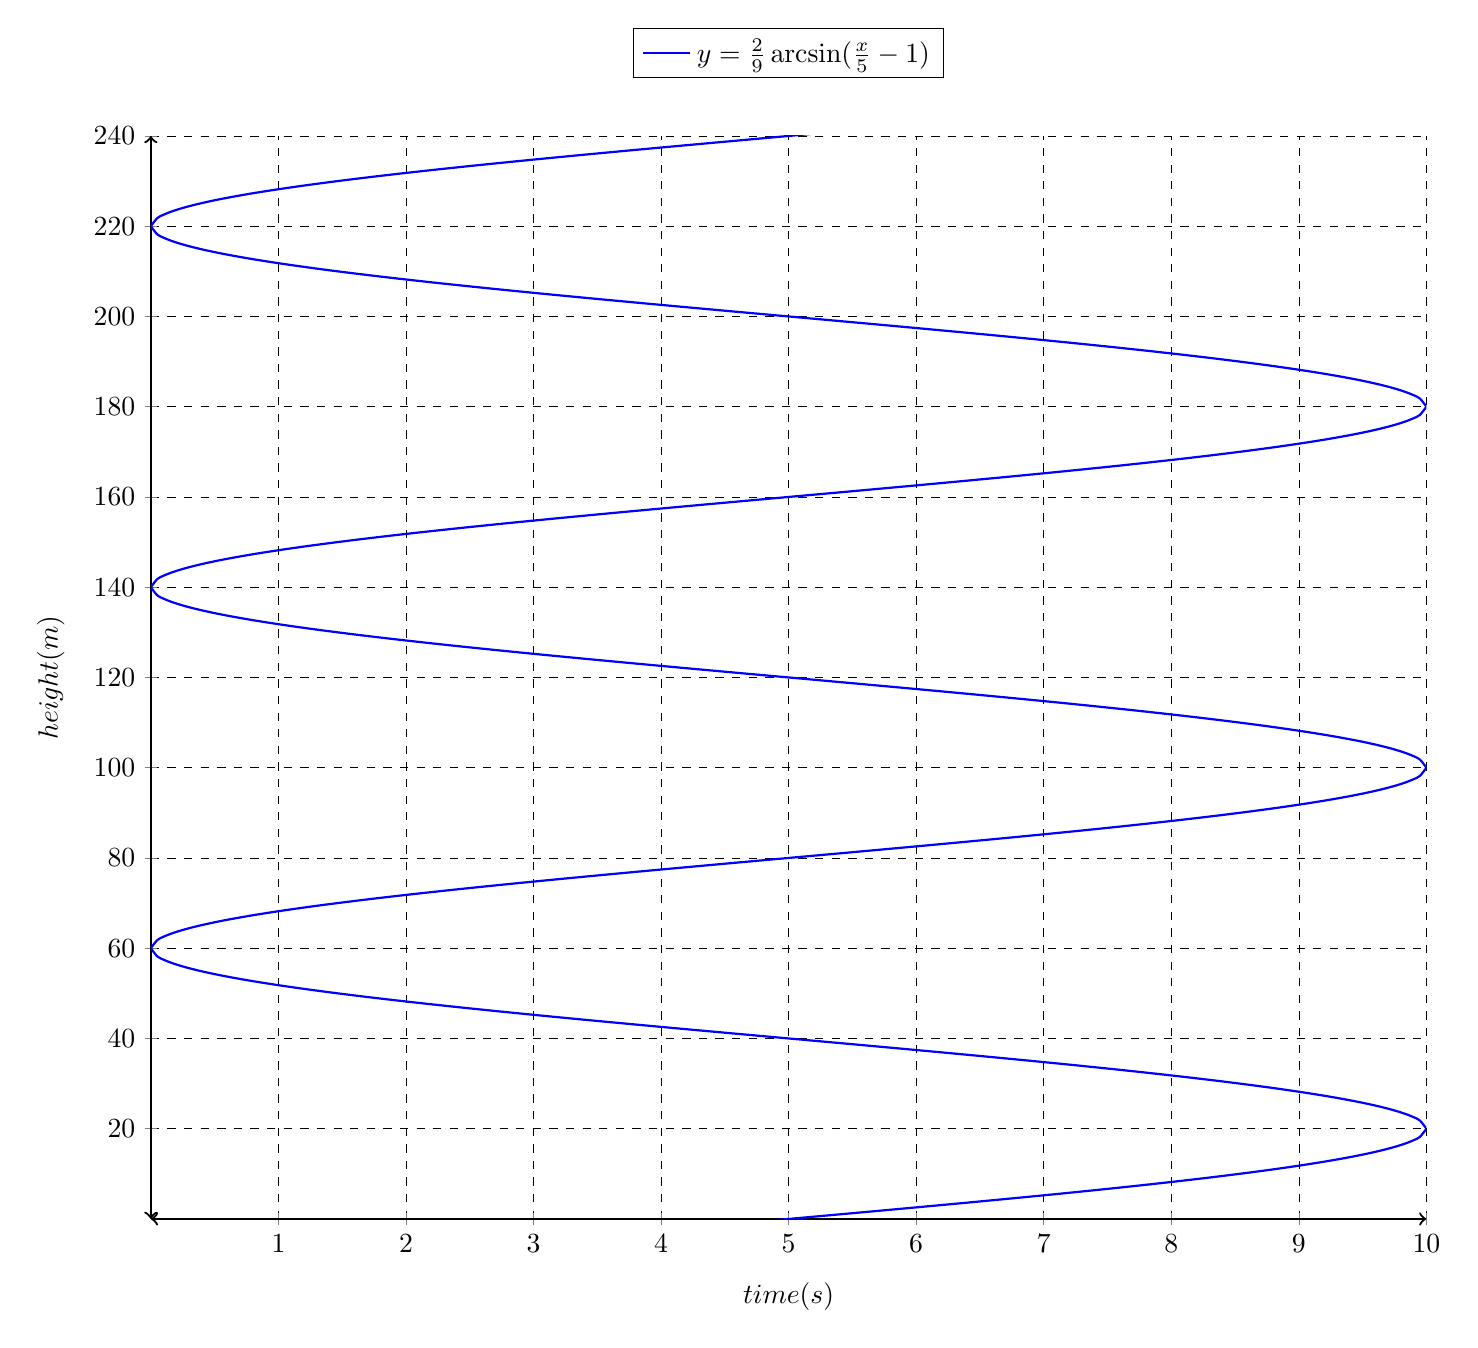
\begin{tikzpicture}
            \begin{axis}[
                axis lines=middle,
                axis line style={thick,<->},
                ymin=0,ymax=240,xmin=0,xmax=10,
                xtick={+1,+2,...,+10},
                ytick={+20,+40,...,+240},
                tick label style={font=\normalsize},
                grid=major,
                major grid style={dashed,very thin,black},
                every axis plot post/.append style={thick},
                label style={font=\normalsize},
                x label style={at={(axis description cs:0.5,-0.05)},anchor=north},
                y label style={at={(axis description cs:-0.06,0.5)},rotate=90,anchor=south},
                xlabel=$time(s)$,
                ylabel=$height(m)$,
                smooth,
                legend style={
                        font=\normalsize,
                        at={(0.5, 1.1)},
                        anchor=north
                        }
                ]
                \addplot[domain=0:10,samples=200,blue] {(2/9)*asin(x/5 - 1)};
                \addplot[domain=0:10,samples=200,blue] {-(2/9)*asin(x/5 - 1) + 40};
                \addplot[domain=0:10,samples=200,blue] {(2/9)*asin(x/5 - 1) + 80};
                \addplot[domain=0:10,samples=200,blue] {-(2/9)*asin(x/5 - 1) + 120};
                \addplot[domain=0:10,samples=200,blue] {(2/9)*asin(x/5 - 1) + 160};
                \addplot[domain=0:10,samples=200,blue] {-(2/9)*asin(x/5 - 1) + 200};
                \addplot[domain=0:10,samples=200,blue] {(2/9)*asin(x/5 - 1) + 240};
                \legend{$y = \frac{2}{9}\arcsin(\frac{x}{5} - 1)$} \\
            \end{axis}
        \end{tikzpicture}
    \end{adjustwidth}
    
    \textbf{f) Is the relation in part e) a function? Justify your answer.} \\
    \text{No, the relation in part e) is not a function, as it does not pass the vertical line test.} \\
\end{adjustwidth}

\textbf{8. Consider what happens to a relation when the coordinatges of all its ordered pairs are switched.} \\
\begin{adjustwidth}{1cm}{0pt}
    \textbf{a) Give an example of a function that is still a function when its coordinates are switched.} \\
    $\{(0,0),(1,1),(4,2)\}$ \\
    \\
    \textbf{b) Give an example of a function that is no longer a function when its coordinates are switched.} \\
    $y = x^2$ \\
    \\
    \textbf{c) Give an example of a relation that is not a function, but becomes a function when its coordinates are switched.} \\
    $y = \pm\sqrt{x}$
\end{adjustwidth}

\textbf{9. Explain why a relation that fails the vertical line test is not a function.} \\
\begin{adjustwidth}{1cm}{0pt}
    a function is an equation or set of ordered pairs where every x-value only 
    cooresponds to one y-value, and when a relation fails the vertical line test,
    it means that a vertical line can be drawn that intersects the graph at more 
    than one point, which means that there is an x value that cooresponds to more 
    than one y-value.
\end{adjustwidth}

\textbf{11. The table below lists all the ordered pairs that belong to the function $g(x)$} \\ \\
\begin{tabular}{| c | c | c | c | c | c | c |}
    \hline
    x & 0 & 1 & 2 & 3 & 4 & 5 \\
    \hline
    $g(x)$ & 3 & 4 & 7 & 12 & 19 & 28 \\
    \hline
\end{tabular}
\\
\begin{adjustwidth}{1cm}{0pt}
    \textbf{a) Determine an equation for $g(x)$} \\
    $g(x) = x^2 + 3$ \\
    \\
    \textbf{b) Does $g(3) - g(2) = g(3 - 2)$? Explain.} \\
    \begin{math}
        g(3) - g(2) = (3^2 + 3) - (2^2 + 3) \\
        g(3) - g(2) = (12) - (7) \\
        g(3) - g(2) = 5 \\
        \\
        g(3 - 2) = (3 - 2)^2 + 3 \\
        g(3 - 2) = (1)^2 + 3 \\
        g(3 - 2) = 4 \\
        \\
        \therefore g(3) - g(2) \neq g(3 - 2) \\
    \end{math}
\end{adjustwidth}
\end{document}